\documentclass[spanish]{article}
\usepackage{csquotes}
\usepackage[spanish]{babel}
\selectlanguage{spanish}
\usepackage[utf8]{inputenc}
\usepackage{authblk}
\usepackage{amsmath}
\usepackage{amsfonts}

\usepackage[
	backend=biber,
	style=numeric,
]{biblatex}

\usepackage{enumitem}
\usepackage{extarrows}
\usepackage{mathtools}
\usepackage{systeme}
\usepackage{graphicx}
\usepackage{float}
\usepackage{listings}
\usepackage{listingsutf8}

\usepackage{multirow}
\usepackage{minted}

\graphicspath{ {./img/} }

%\addbibresource{./sources.bib}

\newcommand{\cimg}[2]{
\begin{figure}[H]
	\center
		\includegraphics[width=#2\linewidth]{#1}
\end{figure}
}

\begin{document}

\begin{titlepage}
	\centering
	{\huge\bfseries Practica 3 - Migración de máquinas virtuales \par}
	\vspace{1cm}
	{\scshape\Large Aurora Zuoris \par\tt{aurora.zuoris101@alu.ulpgc.es}\par}
	\vspace{3cm}
	{\scshape\large Virtualización y Processamiento Distribuido\par}
	\vspace{1cm}
	{\scshape\large Grado en Ciencias e Ingeniería de Datos\par}
	\vspace{1cm}
	{\scshape\large Escuela de Ingeniería Informática\par}
	\vspace{1cm}
	{\scshape\large Universidad de Las Palmas de Gran Canaria\par}
	\vspace{1cm}
	{\scshape\large \today{} \par}
\end{titlepage}

\newpage

\tableofcontents

\newpage

\section{Introducción}

%En este informe se describe como realizar
%varias operaciones con maquinas virtuales.
%Primero se muestra como se copia una maquina virtual a mano, ocn el fin 
%de entender que archivos son necesarios para que una maquina virtual funcione.
%luego se muestra como se copia una maquina virtual con
%las herramientas diseñadas para tal fin,
%Al final se instala una maquina virtual a partir de virt-install.

Este informe se centra sobre la migración de maquinas virtuales.
Esta operación consiste en mover una máquina virutal entre dos anfitriones.
Para esto, se asegura que los dos tengan una connección, se configura SSH para que uno pueda
conectarse al otro, y además hay que tener un NAS montado en ambos anfitriones.

\section{Desarollo}

Lo primero que se hace es asegurarse que ambas máquinas se conecten.
En el caso del desarollo de la práctica, esta se realizó en el laboratorio universitario,
con lo que todas las máquinas estaban en la red de esta.
Es posible obtener la ip de uno mediante el comando \texttt{ip addr},
para ver las IPs asignadas de cada interfaz red.
Se puede verificar que hay conección entre dos máquinas realizando un \texttt{ping} a la dirección del otro.

Para usar nombres en vez de direcciones IPv4, se puede configurar el archivo \texttt{/etc/hosts} para que
el anfitrion resuelva un nombre dado a la dirección IP deseada,
tal que el contenido del archivo contenga una linea como la siguiente.

\texttt{10.22.146.15 pc1165.vpd.com}

Uno también puede configurar las máquinas tal que tengan estos
nombres como su hostname con el uso del comando \texttt{hostnamectl},
pero esto no es necesario e irrelevante en cuanto a conseguir que las
differentes máquinas se accedan mediante un nombre en vez de una dirección IP.

\begin{lstlisting}[language=bash,breaklines=true]
$ hostnamectl set-hostname pc1167.vpd.com
\end{lstlisting}

También hay que asegurarse que ambas máquinas sean autorizadas para comunicarse la una con la otra.
En este caso esto se hace mediante ssh. Primero hay que asegurarse que el servidor, \texttt{sshd}, esté en ejecución.

\begin{lstlisting}[language=bash,breaklines=true]
$ systemctl status sshd
\end{lstlisting}

En el caso de que no lo esté, se puede activar mediante \texttt{systemctl enable --now sshd}.

Para autorizar las máqunias unas con las otras, se crea un par de claves públicas-privadas:

\begin{lstlisting}[language=bash,breaklines=true]
$ ssh-keygen
\end{lstlisting}

Esto creará los archivos \texttt{{\texttildelow}/.ssh/id\_rsa} y \texttt{\texttildelow/.ssh/id\_rsa.pub}. El segundo de estos es la
clave pública, la cual debe concatenarse al archivo \texttt{\texttildelow/.ssh/authorized\_keys} del otro anfitrión.

A continuación, hace falta que ambos anfitriones tengan una NAS montada en el mismo punto de entrada.
Ya que una vez migrada la máquina virtual, hace falta que esta sigua podiendo acceder su disco sin interrupciones.

\begin{lstlisting}[language=bash,breaklines=true]
$ mkdir nas
$ mount -t nfs disnas.dis.ulpgc.es:/disnas-itsi nas
$ virt-clone -o MinimalFedoraServer39 -n AuroraFedoraServer -f /root/nas/pc1167_Lab11_ANFITRION1_practica_migracion.qcow2
\end{lstlisting}

Por último, hace falta que configurar el cortafuegos para que
los puertos por los que se realizarán la migración estén abiertos.
Esto se realiza mediante el comando \texttt{firewall-cmd}:

\begin{lstlisting}[language=bash,breaklines=true]
$ firewall-cmd --permanent --add-port=49152-49216/tcp
$ firewall-cmd --reload
\end{lstlisting}

Una vez todos estos pasos se han realizado, se puede migrar la máquina mediante el virt manager con click derecho sobre la máquina
y usando la opción migrate. Esto se puede ver en la figura \ref{fig:migration}.

\begin{figure}[h]
\centering
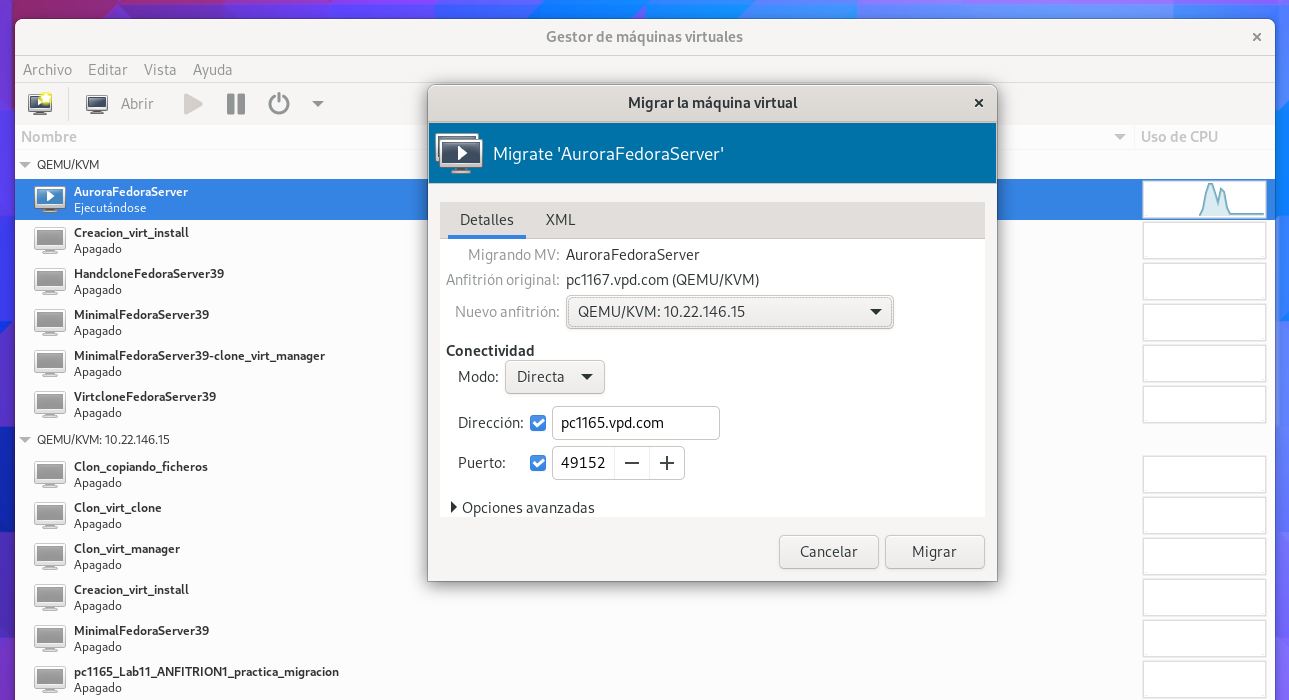
\includegraphics[width=0.8\textwidth]{migration}
\caption{Migración de máquinas virtuales}
\label{fig:migration}
\end{figure}

\section{Pruebas/Validación}

Se puede validar viendo que una vez realizada la migración,
en el virtual manager se puede ver esa misma máquina virtual residiendo en el otro anfitrión.
Esto se puede ver en la Figura \ref{fig:verify}.

\begin{figure}[h]
\centering
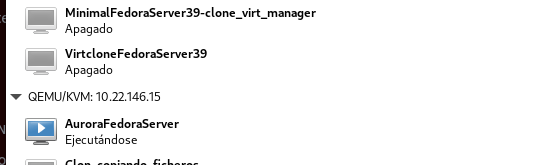
\includegraphics[width=0.8\textwidth]{verification}
\caption{Migración de máquinas virtuales}
\label{fig:verify}
\end{figure}

\end{document}
